% !TEX root = ../main.tex
\chapter{Kiến thức nền tảng}\label{chap:background}

Chương này trình bày các khái niệm và kỹ thuật nền tảng mà hệ thống ARGOS được xây dựng trên đó. Mỗi mục được trình bày ở mức độ đủ để người đọc theo dõi các phân tích kiến trúc ở các chương sau: từ định nghĩa bài toán CRS, cấu trúc Đồ thị tri thức, kỹ thuật LLM và RAG, đến mô hình Đa tác tử và các thang đo đánh giá.

\section{Định nghĩa bài toán Hệ thống Gợi ý Hội thoại (CRS)}
Không giống các hệ thống gợi ý truyền thống vốn chỉ nhận đầu vào là lịch sử tương tác ngầm (implicit feedback), CRS tương tác trực tiếp với người dùng qua ngôn ngữ tự nhiên để khai thác sở thích một cách chủ động \cite{li2018towards, christakopoulou2016towardscrs}. Trọng tâm là khả năng duy trì mạch hội thoại đa lượt: hệ thống đặt câu hỏi để làm rõ nhu cầu (preference elicitation), cập nhật hiểu biết về người dùng sau mỗi lượt và đưa ra gợi ý kèm lý giải thuyết phục. CRS đặc biệt có giá trị trong tình huống cold-start, khi hệ thống chưa có dữ liệu tương tác lịch sử của người dùng mới.

Về kiến trúc, một CRS truyền thống gồm ba module cốt lõi: NLU (Natural Language Understanding) trích xuất ý định, DST (Dialogue State Tracking) theo dõi trạng thái hội thoại, và NLG (Natural Language Generation) sinh phản hồi.

Bài toán CRS được hình thức hóa như sau: cho tập item $\mathcal{I}$ và ngữ cảnh hội thoại tại lượt $t$, $C_t = \{u_1, s_1, \dots, u_t\}$, trong đó $u_i$ là phát ngôn người dùng và $s_i$ là phản hồi hệ thống ở lượt $i$, hệ thống thực hiện hai nhiệm vụ song song:
\begin{enumerate}
    \item \textbf{Gợi ý (Recommendation):} Dự đoán tập con $I_{rec} \subset \mathcal{I}$ phù hợp nhất với hồ sơ sở thích động của người dùng, liên tục cập nhật theo phản hồi chấp nhận/từ chối ở các lượt trước.
    \item \textbf{Sinh hội thoại (Dialogue Generation):} Sinh phản hồi $s_t$: hoặc là câu hỏi khai thác thêm thông tin khi độ tin cậy chưa đủ, hoặc là lời giới thiệu tích hợp các item trong $I_{rec}$ cùng lý do giải thích để tăng mức độ tin tưởng của người dùng.
\end{enumerate}

Hình \ref{fig:crs_dialogue_example} minh họa một đoạn hội thoại CRS điển hình, cho thấy hệ thống luân phiên đặt câu hỏi khai thác sở thích và đưa ra gợi ý qua nhiều lượt trao đổi với người dùng.

\begin{figure}[htbp]
    \centering
    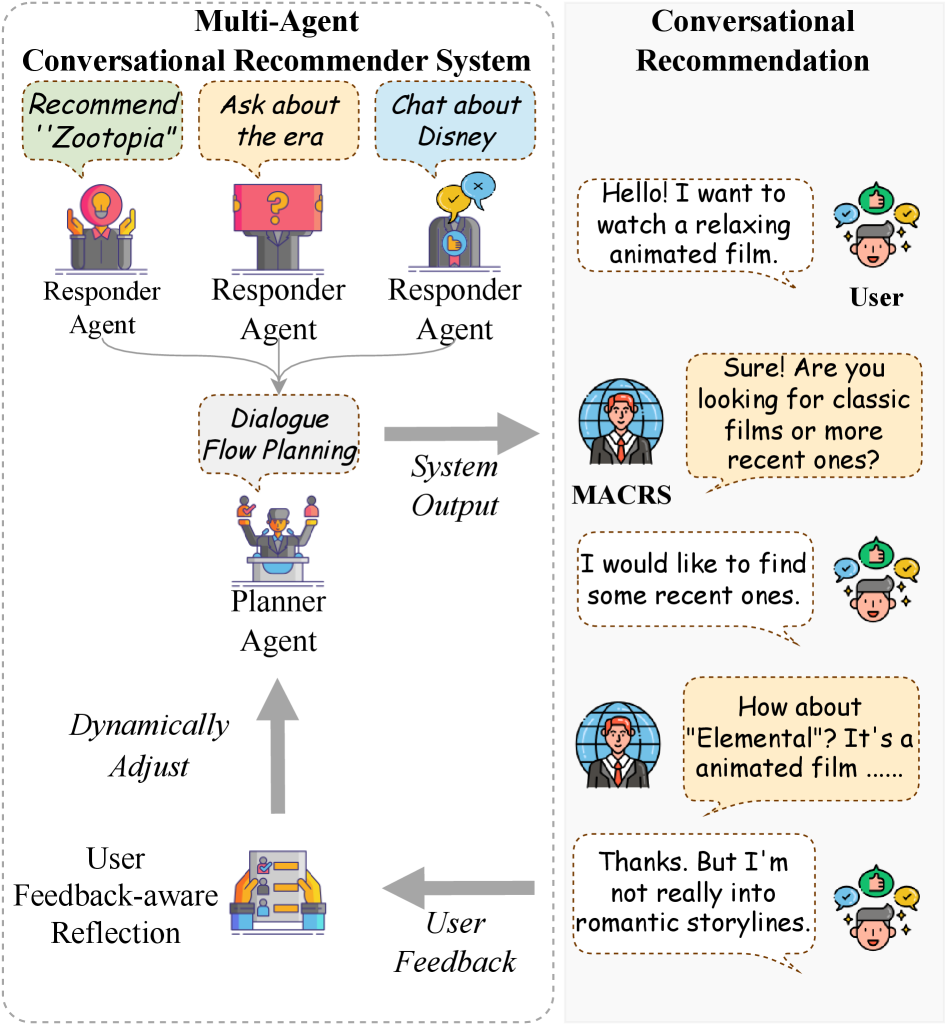
\includegraphics[width=\linewidth]{Chap2/images/crs_dialogue_example.png}
    \caption{Ví dụ hội thoại nhiều lượt trong Hệ thống gợi ý hội thoại. Hệ thống chủ động đặt câu hỏi làm rõ sở thích, cập nhật trạng thái hội thoại và đưa ra gợi ý kèm giải thích qua từng lượt tương tác \cite{fang2024multiagentconversationalrecommender}.}
    \label{fig:crs_dialogue_example}
\end{figure}

\section{Đồ thị Tri thức (Knowledge Graph - KG)}
Đồ thị tri thức (KG) biểu diễn tri thức thực thể dưới dạng tập hợp các bộ ba có hướng:
\begin{equation}
    \mathcal{G} = \{(h, r, t) \mid h, t \in \mathcal{E}, r \in \mathcal{R}\}
\end{equation}
trong đó $\mathcal{E}$ là tập thực thể (Phim, Đạo diễn, Thể loại, Diễn viên), $\mathcal{R}$ là tập quan hệ (đạo\_diễn\_bởi, thuộc\_thể\_loại, đóng\_vai), $h$ (head) và $t$ (tail) là thực thể gốc và đích, $r$ là quan hệ có hướng nối giữa chúng \cite{zhou2020improvingcrs}.

Trong ngữ cảnh CRS, dữ liệu tương tác người dùng - item thường rất thưa thớt (data sparsity). KG đóng ba vai trò bổ sung mà lịch sử tương tác đơn thuần không thể cung cấp:
\begin{itemize}
    \item \textbf{Nguồn dữ liệu thực chứng (Grounding):} Mọi thực thể được gợi ý đều có thể kiểm tra sự tồn tại trực tiếp trong KG, là nền tảng để loại bỏ hallucination từ LLM.
    \item \textbf{Suy luận đa bước (Multi-hop Reasoning):} Duyệt qua các cạnh đồ thị ở độ sâu $> 1$ cho phép phát hiện sở thích tiềm ẩn mà lịch sử tương tác trực tiếp không thể hiện (ví dụ: Phim $\rightarrow$ Diễn viên $\rightarrow$ Phim khác cùng diễn viên).
    \item \textbf{Nền tảng cho Truy xuất lai (Hybrid Retrieval):} KG hiện đại lưu trữ song song cả liên kết cấu trúc và vector nhúng (embeddings) của nội dung văn bản (tóm tắt cốt truyện, mô tả thực thể), cho phép kết hợp truy xuất ngữ nghĩa và truy xuất đồ thị trong cùng một hệ thống.
\end{itemize}

Hình \ref{fig:kg_structure_bg} minh họa cụ thể cách một node Phim được tổ chức trong KG, với các cạnh có hướng nối tới các thực thể liên quan như Đạo diễn, Diễn viên và Thể loại, thể hiện trực quan cấu trúc bộ ba $(h, r, t)$ được định nghĩa ở trên.

\begin{figure}[htbp]
    \centering
    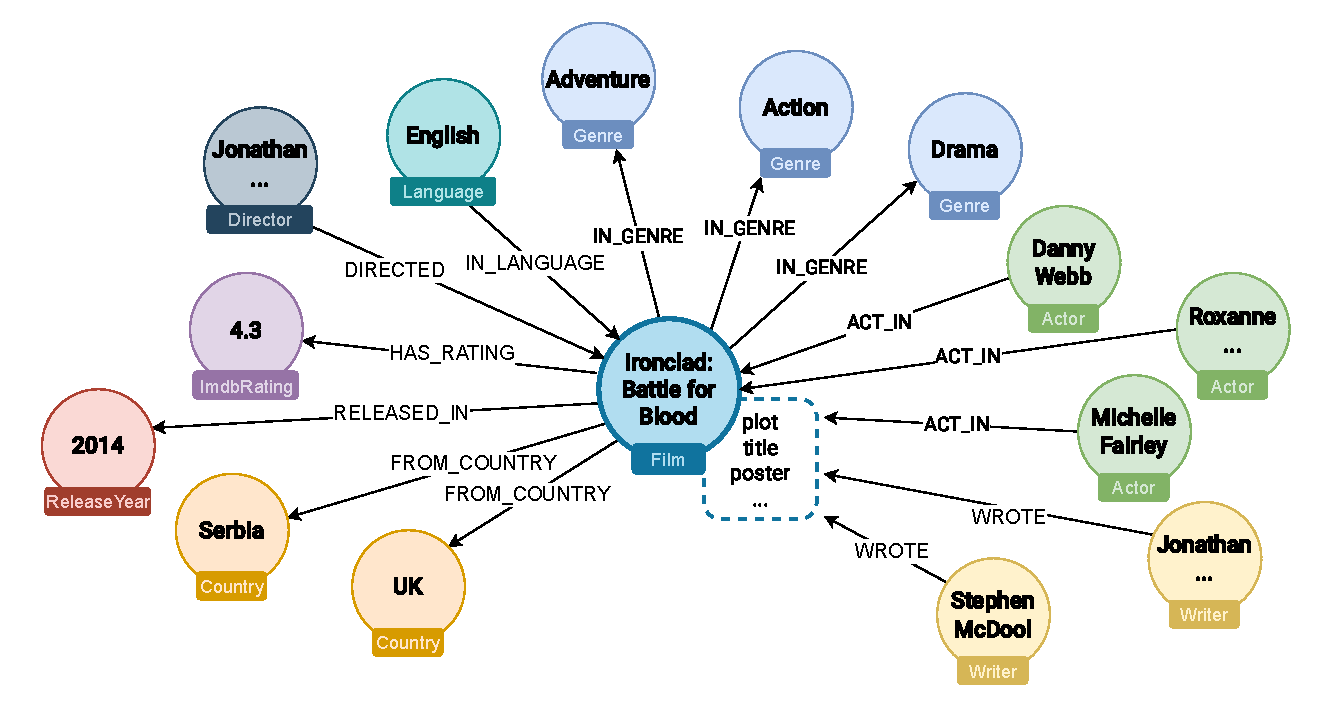
\includegraphics[width=0.75\linewidth]{Chap3/images/KG_node.pdf}
    \caption{Ví dụ cấu trúc một node Phim trong Đồ thị tri thức, liên kết với các thực thể Đạo diễn, Diễn viên, Thể loại và các thuộc tính định lượng. Mỗi bộ ba $(h, r, t)$ biểu diễn một quan hệ có hướng giữa hai thực thể trong đồ thị.}
    \label{fig:kg_structure_bg}
\end{figure}

\section{Mô hình Ngôn ngữ Lớn (LLMs) và Kỹ thuật RAG}

\subsection{Mô hình Ngôn ngữ Lớn (LLMs)}
LLM là các mô hình Transformer được huấn luyện trên khối lượng văn bản khổng lồ, có khả năng hiểu và sinh ngôn ngữ tự nhiên theo ngữ cảnh \cite{min2023recent}. Trong hệ thống CRS, LLM đảm nhận ba chức năng chính: (1) phân tích ý định và trích xuất ràng buộc từ lịch sử hội thoại, (2) suy luận về độ phù hợp của các ứng viên, và (3) sinh phản hồi ngôn ngữ tự nhiên \cite{zhao2024recommender}.

Hạn chế căn bản của LLM trong CRS là \textit{hallucination}: vì sinh văn bản theo phân phối xác suất, LLM có thể tự tạo ra các thực thể không tồn tại (phim bịa, đạo diễn sai) nhưng hoàn toàn hợp lý về mặt ngôn ngữ. Đây là lý do cần neo giữ (ground) đầu ra của LLM vào một nguồn dữ liệu thực chứng bên ngoài, vai trò mà KG đảm nhận trong hệ thống ARGOS.

\subsection{Kỹ thuật RAG (Retrieval-Augmented Generation)}
RAG giải quyết hạn chế của LLM bằng cách tách biệt lưu trữ tri thức (trong cơ sở dữ liệu ngoài) khỏi năng lực suy luận (của LLM) \cite{singh2026agenticretrievalaugmentedgenerationsurvey}. Thay vì học thuộc dữ liệu vào trọng số, LLM nhận tri thức liên quan theo thời gian thực qua hai pha:
\begin{enumerate}
    \item \textbf{Truy xuất (Retrieval):} Dựa trên truy vấn $q$, tìm kiếm tập tài liệu/thực thể $D$ liên quan từ kho dữ liệu ngoài (KG, vector database).
    \item \textbf{Sinh có điều kiện (Conditioned Generation):} LLM sinh phản hồi dựa trên $q$ và $D$ kết hợp, câu trả lời được neo giữ vào dữ liệu thực chứng thay vì chỉ dựa vào phân phối tham số.
\end{enumerate}

Luồng hoạt động tổng thể của pipeline RAG được minh họa trong Hình \ref{fig:rag_pipeline}.

\begin{figure}[htbp]
    \centering
    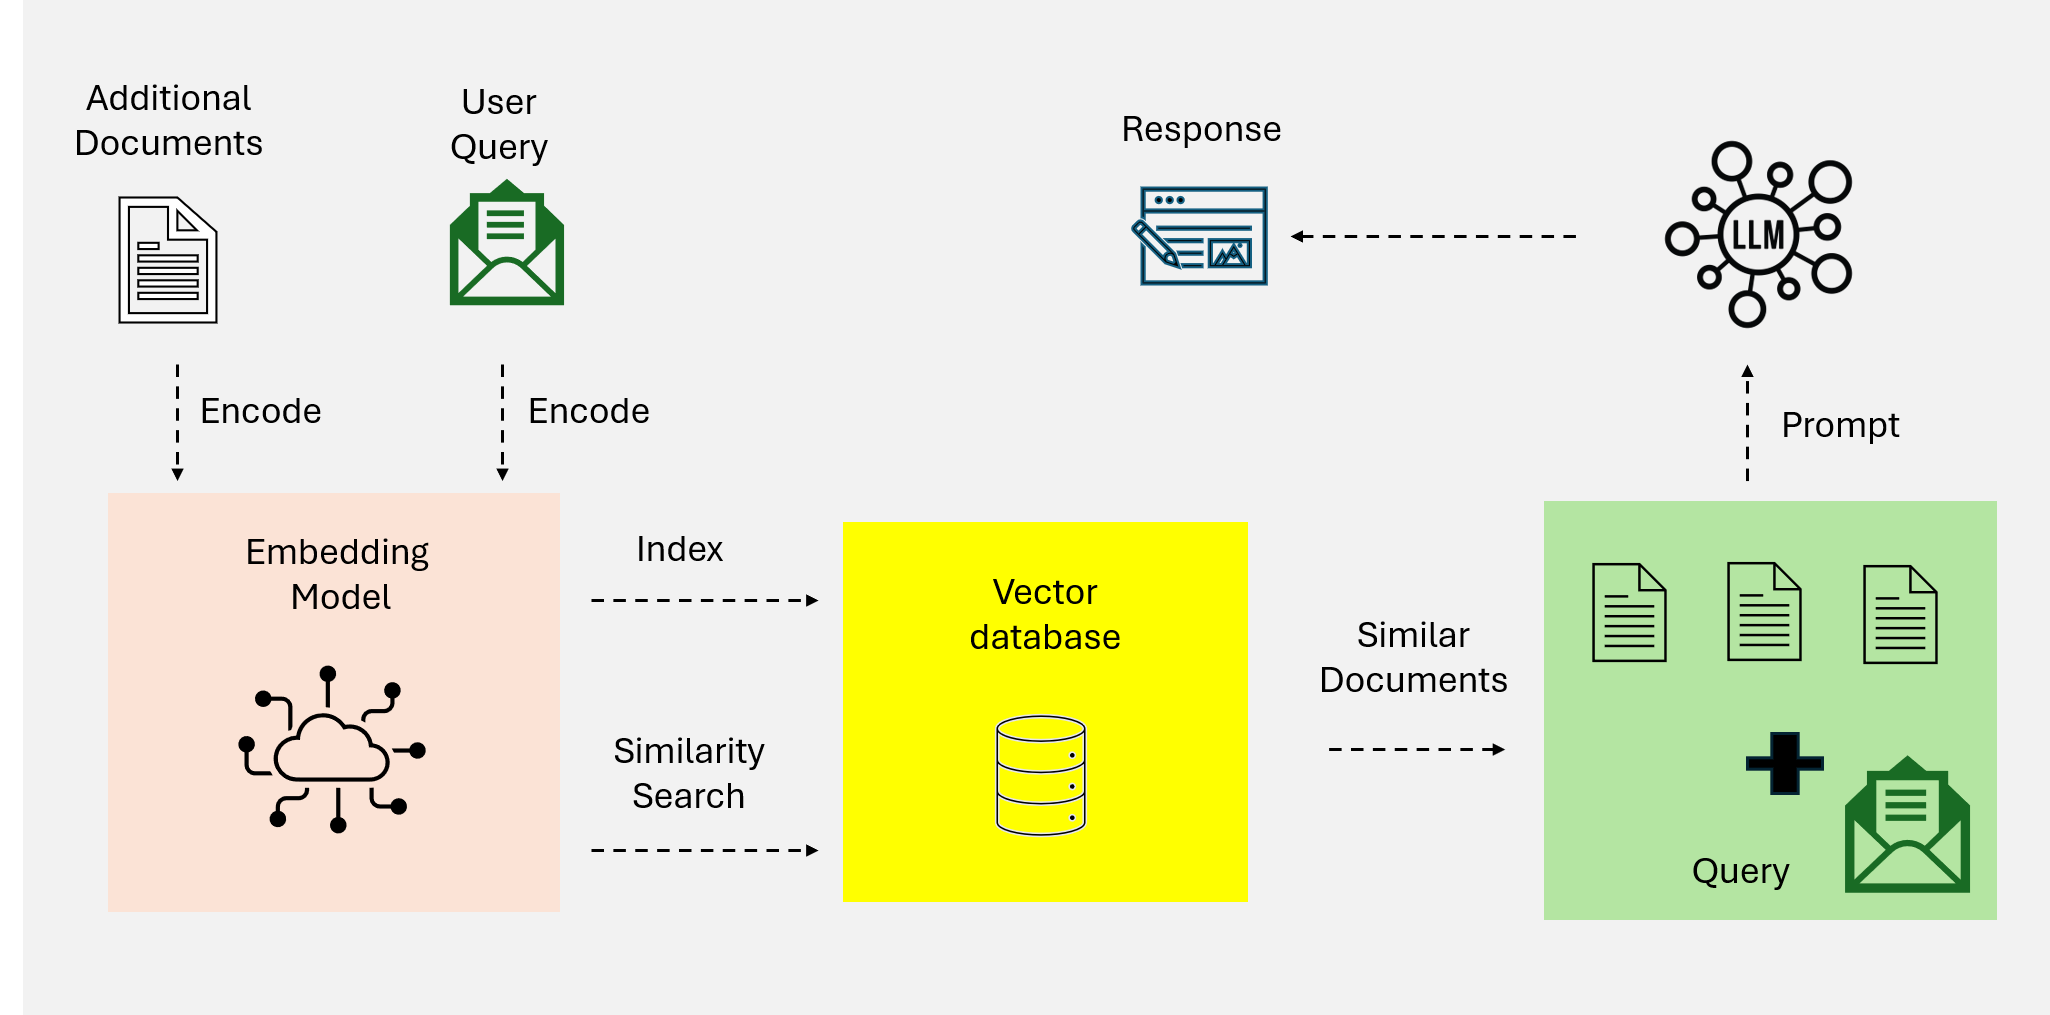
\includegraphics[width=\linewidth]{Chap2/images/rag_pipeline.png}
    \caption{Pipeline RAG cơ bản gồm ba giai đoạn: \textit{Retrieval} (truy xuất tài liệu liên quan từ kho dữ liệu ngoài), \textit{Augmentation} (tích hợp tài liệu vào ngữ cảnh) và \textit{Generation} (LLM sinh câu trả lời được neo giữ vào dữ liệu thực chứng) \cite{singh2026agenticretrievalaugmentedgenerationsurvey}.}
    \label{fig:rag_pipeline}
\end{figure}

RAG đặc biệt phù hợp với bài toán CRS vì ba lý do thực tiễn: (i) danh mục item thay đổi liên tục: RAG chỉ cần cập nhật KG mà không cần fine-tune lại LLM; (ii) mỗi gợi ý đều cần có cơ sở thực chứng: đường dẫn truy xuất của RAG cung cấp trực tiếp khả năng giải thích (explainability); (iii) chi phí thấp hơn đáng kể so với fine-tuning khi quy mô dữ liệu lớn.

\section{Kiến trúc Hệ thống Đa tác tử (Multi-Agent System) và ReAct}

\subsection{Hệ thống Đa tác tử dựa trên LLM}
Kiến trúc đa tác tử dựa trên LLM phân tách một hệ thống phức tạp thành nhiều tác tử (agents) tự trị, mỗi tác tử chuyên trách một nhiệm vụ cụ thể với prompt riêng và quyền truy cập vào các công cụ được chỉ định \cite{xi2023rise}. Nghiên cứu gần đây cho thấy cách tiếp cận này vượt trội so với kiến trúc đơn tác tử trong các bài toán đòi hỏi phân tích đa chiều, tự sửa lỗi và phối hợp giữa các nguồn thông tin dị dạng, đặc điểm phù hợp với tính chất phức tạp của hội thoại gợi ý thực tế.

\subsection{Vòng lặp ReAct (Reasoning and Acting)}
ReAct \cite{yao2022react} là framework cho phép tác tử xen kẽ giữa suy luận (Thought) và hành động tương tác với môi trường (Action-Observation) trong một vòng lặp liên tục:
\begin{itemize}
    \item \textbf{Thought:} Tác tử phân tích trạng thái hiện tại và lập kế hoạch bước tiếp theo.
    \item \textbf{Action:} Gọi công cụ cụ thể (truy vấn KG, gọi API) với tham số phù hợp.
    \item \textbf{Observation:} Nhận kết quả từ công cụ, cập nhật ngữ cảnh và lặp lại.
\end{itemize}

Hình \ref{fig:react_loop} so sánh trực quan vòng lặp ReAct với các phương pháp prompting khác, làm rõ cách xen kẽ giữa Thought và Action-Observation tạo nên khả năng tự điều chỉnh mà các phương pháp đơn thuần không có.

\begin{figure}[htbp]
    \centering
    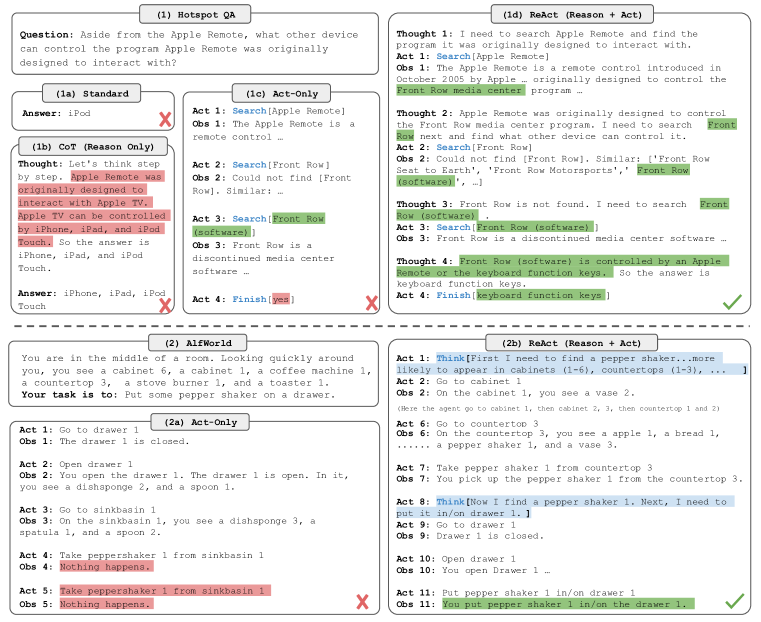
\includegraphics[width=\linewidth]{Chap2/images/react_loop.png}
    \caption{So sánh các phương pháp prompting LLM: Standard, Chain-of-Thought, Act-only và \textbf{ReAct}. ReAct xen kẽ giữa suy luận (Thought) và hành động tương tác với môi trường (Action-Observation), cho phép tác tử tự điều chỉnh chiến lược dựa trên phản hồi từ môi trường \cite{yao2022react}.}
    \label{fig:react_loop}
\end{figure}

ReAct phù hợp đặc biệt với bài toán CRS vì bản chất tương tác đa lượt của hội thoại đòi hỏi hệ thống phải liên tục quan sát, điều chỉnh, hành động trong vòng lặp, chứ không thể xử lý một lần rồi kết thúc như pipeline tĩnh. Cụ thể, khi một bước truy xuất KG thất bại, ReAct cho phép tác tử nhận biết sự cố qua Observation, suy luận nguyên nhân qua Thought tiếp theo, và thử chiến lược truy xuất khác qua Action mới, thay vì dừng hẳn và trả về kết quả rỗng. Đây chính xác là cơ chế mà các pipeline tĩnh đang thiếu.

\section{Bộ dữ liệu thực nghiệm}

Toàn bộ quá trình đánh giá trong khóa luận sử dụng hai bộ dữ liệu hội thoại chuẩn của lĩnh vực CRS:

\textbf{ReDial} \cite{li2018towards} là bộ dữ liệu hội thoại gợi ý phim tiếng Anh được thu thập qua Amazon Mechanical Turk, gồm hơn 10.000 hội thoại đa lượt giữa người hỏi và người trả lời. Mỗi hội thoại chứa ít nhất một lượt gợi ý phim với nhãn xác nhận (accepted/rejected), tạo thành ground truth rõ ràng cho đánh giá Recall@K.

\textbf{INSPIRED} \cite{hayati-etal-2020-inspired} là bộ dữ liệu hội thoại gợi ý phim tập trung vào chiến lược thuyết phục xã hội (social influence strategies), gồm 1.001 hội thoại với ngôn ngữ tự nhiên, cảm xúc và phong cách giao tiếp đa dạng hơn ReDial. Bộ dữ liệu này kiểm tra khả năng hiểu ngôn ngữ linh hoạt và hội thoại phi cấu trúc của hệ thống.

Hai bộ dữ liệu bổ sung cho nhau: ReDial đánh giá hiệu năng ở quy mô lớn với phân phối cân bằng, còn INSPIRED kiểm tra khả năng xử lý các truy vấn cảm xúc và ngôn ngữ đời thường. Giao thức đánh giá chi tiết (chiến lược lấy mẫu, kiểm định thống kê) được trình bày trong Chương 5.

\section{Các phương pháp đánh giá hệ thống (Evaluation Metrics)}
Nghiên cứu này sử dụng thang đo tiêu chuẩn \textbf{Recall@K} trong lĩnh vực gợi ý để đánh giá module Recommendation của ARGOS. Thang đo này phù hợp với bài toán CRS vì mỗi lượt hội thoại thường chỉ có một mục ground truth duy nhất, nên việc đo tỷ lệ xuất hiện trong top-K là chỉ số đánh giá trực tiếp và có ý nghĩa nhất.

\textbf{Recall@K} đo tỷ lệ item mục tiêu (ground truth) xuất hiện trong top-K gợi ý. Ký hiệu $V_u$ là tập item thực tế người dùng quan tâm, $R_u@K$ là top-K gợi ý của hệ thống:
\begin{equation}
    \text{Recall@K} = \frac{1}{|U|} \sum_{u \in U} \frac{|R_u@K \cap V_u|}{|V_u|}
\end{equation}

Thang đo được tính tại bốn ngưỡng $K \in \{1, 5, 10, 50\}$ trên hai bộ dữ liệu chuẩn ReDial \cite{li2018towards} và INSPIRED \cite{hayati-etal-2020-inspired}, nhất quán với giao thức đánh giá của các hệ thống SOTA được đối sánh trong Chương 5.

\section*{Kết luận chương}

Chương 2 đã thiết lập bốn nhóm kiến thức cốt lõi phục vụ cho việc hiểu và đánh giá hệ thống ARGOS. Bài toán CRS xác lập không gian vấn đề với hai nhiệm vụ song song mà ARGOS phải giải quyết. Đồ thị tri thức là nguồn dữ liệu thực chứng trung tâm, đảm bảo mọi gợi ý đều có cơ sở kiểm chứng và là nền tảng cho Hybrid Retrieval. LLM kết hợp RAG cung cấp năng lực suy luận ngôn ngữ mà không cần fine-tuning khi dữ liệu thay đổi. Kiến trúc đa tác tử với ReAct là mô hình tổ chức cho phép thiết lập vòng lặp phản hồi nội bộ, thành phần then chốt mà các hệ thống RAG tĩnh đang thiếu, và là nền tảng kỹ thuật của ARGOS.

Chương 3 tiếp theo phân tích chi tiết mô hình tiền đề GRACE, nơi RAG kết hợp KG lần đầu được áp dụng vào CRS của chính tác giả, để định lượng chính xác các điểm nghẽn mà ARGOS cần khắc phục.
